\documentclass[conference]{IEEEtran}
% \IEEEoverridecommandlockouts
% The preceding line is only needed to identify funding in the first footnote. If that is unneeded, please comment it out.
\usepackage{cite}
\usepackage{amsmath,amssymb,amsfonts}


\usepackage{hyperref}
%\usepackage[ngerman]{cleveref}
\usepackage[english]{cleveref}

% \usepackage{algorithmic}
\usepackage{graphicx}
\usepackage{textcomp}
\usepackage{xcolor}
\def\BibTeX{{\rm B\kern-.05em{\sc i\kern-.025em b}\kern-.08em
    T\kern-.1667em\lower.7ex\hbox{E}\kern-.125emX}}
\begin{document}

\title{Text Analytica: cloud-based document analysis\\}

\author{\IEEEauthorblockN{Florian Bauer}
\IEEEauthorblockA{\textit{Department of Computer Science} \\
\textit{University of Bristol}\\
Bristol, United Kingdom \\
ya18048@bristol.ac.uk}
\and
\IEEEauthorblockN{Nathalie Pett}
\IEEEauthorblockA{\textit{Department of Computer Science} \\
\textit{University of Bristol}\\
Bristol, United Kingdom \\
aq18034@bristol.ac.uk}
}

\maketitle

\begin{abstract}
The source code is available at https://github.com/darkcookie298/CloudComputing. The application can be run online at http://textanalytica.lukaspman.io/.
\end{abstract}

\section{Introduction}
\label{sec:intro}
Text Analytica is a cloud-based application which aims to support the analysis of text documents. For the purpose of this coursework a prototype has been developed and deployed using different cloud computing technologies. In the remainder of this \Cref{sec:intro}, the general concept behind Text Analytica is discussed as well as the limitations of the implemented prototype. The \Cref{sec:platform-choice} of this report explores the reasons behind choosing \textit{Microsoft's cloud services} over \textit{Oracle's}. Afterwards in \Cref{sec:system-architecture} the system architecture and technologies used for the project are explained in more detail. The scalability of the developed solution is addressed in \Cref{sec:scalability}, including evidence of the performance of the service under load. Lastly, in \Cref{sec:future-improvements}, future improvements of the application are proposed.

\begin{figure*}[ht!]
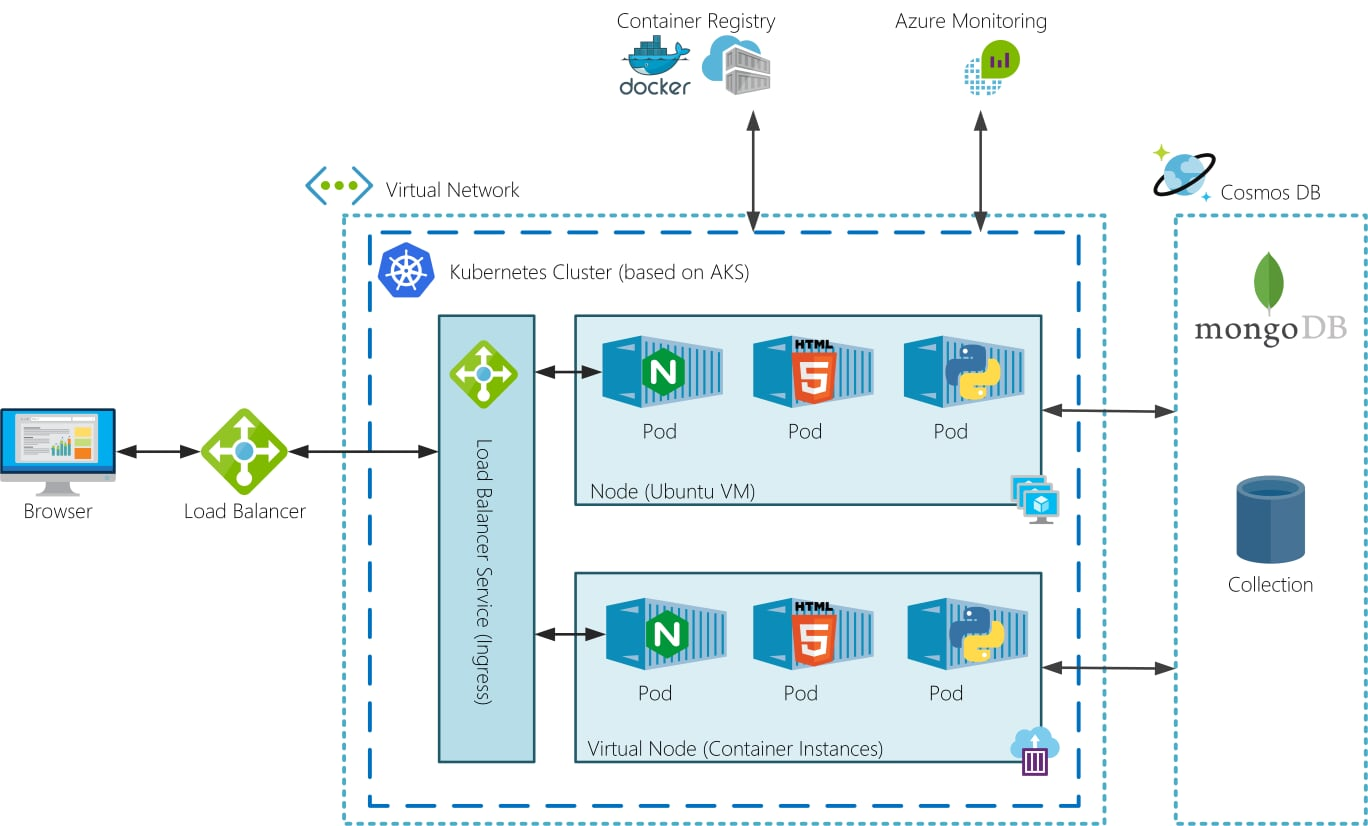
\includegraphics[width=150mm]{img/architecture.jpeg}
\caption{System architecture of our Kubernetes cluster.}
\label{img:architecture}
\end{figure*}

\subsection{Vision}
University students are often faced with an abundance of resources regarding specific units or even certain topics within a unit. These range from lecture notes or slides to personal notes and additional scientific papers as well as e-books or extracts thereof. The first step in the exploration process is for students to familiarize themselves with these materials by identifying the documents’ key aspects and discovering links between different sources. This is what Text Analytica ultimately aims to facilitate.

More specifically the functionalities of Text Analytica could include tagging, keyword search, suggestions of related documents based on textual analysis and eventually the generation of short summaries, all based on user-supplied PDF documents. These functionalities render Text Analytica a useful tool for a large number of scenarios in which people are confronted with many different and possibly complex text sources, e.g. in the context of management decisions in industry or business / commerce.

\subsection{Limitations of the submitted prototype}
\label{subsec:limits}
The focus of this coursework assignment was to deploy an application using different cloud services and explore its scalability. Therefore the functionality of the submitted Text Analytica prototype was stripped down to a minimum.

To skip the step of extracting machine readable text from PDFs by applying OCR techniques, currently users are only able to upload simple .txt documents. These files are then parsed and analyzed. At this point the analysis merely tags the system entries with the three most used nouns in the text. As the current state of analysis functionality does not require the files to be stored within the application (TODO: actually at the moment the whole text is stored in the db), they are discarded after being processed. Additionally the user account and login functionality has not yet been implemented.

\begin{itemize}
	\item explain what we actually implemented and how it is different from the proposed application in FA2 (point to section about improvements)
\end{itemize}

\section{Platform choice}
\label{sec:platform-choice}
The considerations detailed below led to choosing to work with \textit{Microsoft Azure} to remain within the given time scope for the coursework.

\subsection{Setup}
\label{subsec:setup}
At first we tried to use the \textit{Oracle Cloud} and to build and maintain a Kubernetes cluster we wanted to use the \textit{Terraform} command line tool. This was the recommended way we got from the Oracle's Team tutorials in class and for this we had an amount of $3500\pounds$ free credits for the \textit{Oracle Cloud}.
After a long period of installing all needed tools e.g. \textit{Terraform} itself, \textit{Terraform Provider OCI}\cite{TerraformProviderOCI}, \textit{Terraform Kubernetes Installer for Oracle Cloud} \cite{TerrafromK8sInstaller}, we tried to create an easy example cluster.
But already at this point we run into service limits. These limits are restrictions on how many instances of a specific resource in a zone you are allowed to use. To increase the limit you have to open a ticket request and after a few days there will be an Oracle support guy helping you. As the ticket request system is very inconvenient and complicated, and the whole process takes several days this is a very strong
disadvantage of the \textit{Oracle Cloud} in comparison to \textit{Microsoft's Azure}.

The second point of inconvenience using \textit{Oracle Cloud} is the unstructured and inconsistent UI of the control panel, where you can setup and maintain all Oracle services. Especially in comparison to other UIs, e.g. Amazon's, which we discovered in the lecture, and Microsoft's, which we used finally to configure the cluster and database for our cloud application.

\subsection{Documentation and support}
\label{subsec:docandsupport}
An even bigger advantage of using one of \textit{"the big three"} in the cloud business, so \textit{Google Cloud}, \textit{Amazon AWS} or \textit{Microsoft Azure}, is there are a lot of tutorials, answered questions on \textit{Stackoverflow}, etc and better documentations. Respectively using Oracle's cloud leads to
a very small number of tutorials, which is one of the reasons why it is more difficult for beginners. There were a lot of errors or bugs when running their example code, too, but searching for solutions of the problems with \textit{Terraform} and \textit{Oracle Cloud} was very unsuccessful and often ends in no results or other users' questions having the same problems.
So after increasing the service limits and running into errors again and again, we got to a point, where we decided to switch to \textit{Microsoft Azure} and deploy the cloud application Text Analytica there.
In retrospect this was one of our best decisions of the whole project.

\subsection{More Advantages}
In addition to the advantages mentioned in \Cref{subsec:setup} and \Cref{subsec:docandsupport}, there are some more reasons why we decided to migrate the project to Azure:
There is an option to use so called \textit{Virtual Nodes} respectively \textit{Virtual Kubelets}, which fasten scaling times. The functionality and how this is used in the Kubernetes cluster is explained in \Cref{sec:system-architecture}.
Finally there is a bigger community and probably more jobs for the Azure Cloud Services, so it is more meaningful for us to gain experience with this cloud provider instead of Oracle Cloud.

\section{System architecture and service implementation}
\label{sec:system-architecture}
\Cref{img:architecture} shows the architecture of the implemented system, which is discussed in the first two parts of this section in more detail. Text Analytica's two main components are a Kubernetes cluster, managed by the \textit{Azure Kubernetes Service (AKS)} \cite{AKS} and an \textit{Azure Cosmos DB} \cite{CosmosDB}, storing the results of the analysis. In the last part of this section, the service, its underlying code and the continuous integration pipeline used to deploy the application are presented.

\begin{figure*}[ht!]
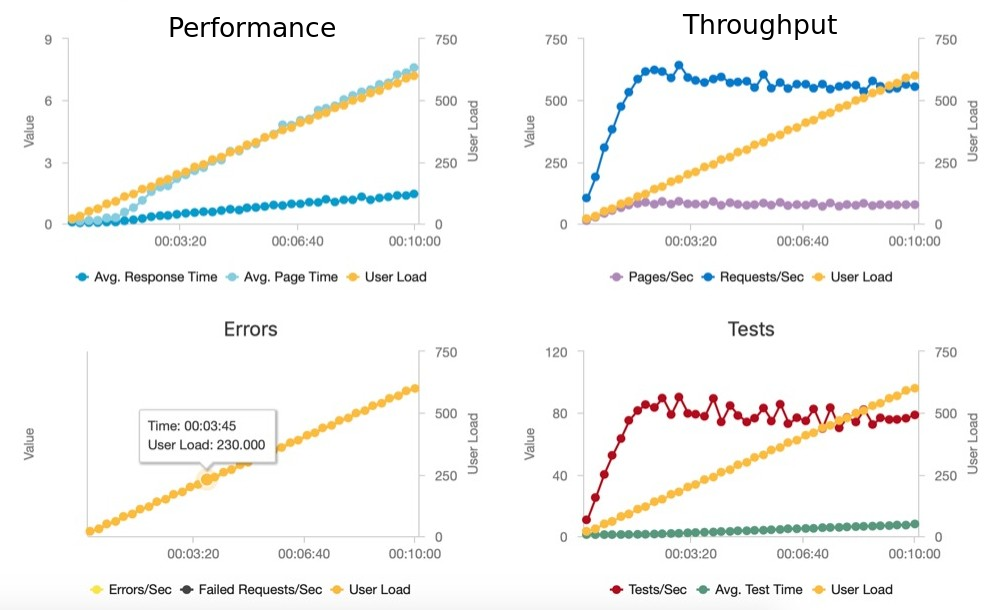
\includegraphics[width=170mm]{img/loadtest_01.png}
\caption{Load tests of the Kubernetes cluster.}
\label{img:loadtesting}
\end{figure*}

\subsection{Infrastructure}
\label{subsec:infra}
Text Analytica’s front-end, back-end and analysis service are currently run within a single Docker container. Container orchestration is handled by a Kubernetes cluster managed by AKS, where each container is encapsulated by a Kubernetes pod. When a new pod is started up the corresponding container is created from a container image pulled from the container registry \textit{Docker Hub}\cite{DockerHub}.

The Kubernetes master node, responsible for the cluster operation, is fully managed by AKS. In addition to the master node the cluster consists of two worker nodes. The first one is based on a general purpose Linux VM, while the second is implemented as a virtual node based on \textit{Azure Container Instances (ACIs)} \cite{AzureContainerInstances} and the \textit{Virtual Kubelet open source project} \cite{VirtualKubelet} \cite{VirtualKubeletGithub}. Kubernetes treats the ACIs compromising the virtual node like standard nodes, so new pods can simply be provisioned on them. Based on container images, ACIs are ready to use in a few seconds as no virtual machines have to be started up and managed by the user. In terms of service level they could be described as \textit{“containers-as-a-service”}.

The cluster is monitored using \textit{Azure Monitor} \cite{AzureMonitor}, a collection of tools to monitor, query and log services and infrastructure running on Azure. It monitors the health of the cluster itself, its nodes and the running services and containers.

To make the pods containing the containerized application available to the public several network measures are in place \cite{AKSNetworks} \cite{AzureExposeKubernetesCluster}. First, a Kubernetes service of type \textit{NodePort} has been created to allow access to the pods via IP address or DNS name and port. To expose the services of Text Analytica for external access an \textit{ingress service} was used. Next to application level load balancing – which at this point is not necessary for Text Analytica, as its services still all run within a single container – ingress can for example be used for SSL / TLS termination. Next to the ingress service an \textit{NGINX ingress controller} is deployed as a pod to each node. The ingress service is of type \textit{LoadBalancer}, which leads Azure to create and configure an \textit{Azure Load Balancer} resource with a corresponding external IP address.

\subsection{Data storage}
As mentioned in \Cref{subsec:limits} currently the only user data stored by Text Analytica are the results of the analysis and related metadata. This data is combined into a json object and sent to the Cosmos DB.

Cosmos DB is a \textit{“globally-distributed, multi-model database”} \cite{CosmosDB}. It was chosen for this project, because it is very easy to set up from the Azure portal, is fully managed and scaled by Azure and can be treated like a MongoDB in development using an API \cite{CosmosMongoDB}.

To provide persistent storage not affected by dying and restarting containers, the database is decoupled from the Kubernetes cluster.

The data in the database is shielded from unwanted access, as it is only accessible from the virtual network in which the Kubernetes cluster is hosted.

\subsection{Service implementation}
•	Front-end built from template using vue.js and bootstrap \cite{Bootstrap}.

•	Backend built with Python using the Flask framework based on several tutorials

•	We used Azure Devops to setup a continuous delivery pipeline to adapt the concept of DevOps. If new code is pushed to the git repository of text analytica, then a new docker container is built automatically and pushed to the docker hub registry. Afterwards the updated containers are applied onto the AKS cluster. The described steps are performed by an Azure pipeline, a service of Azure devops to create build pipelines.

\begin{figure*}[ht!]
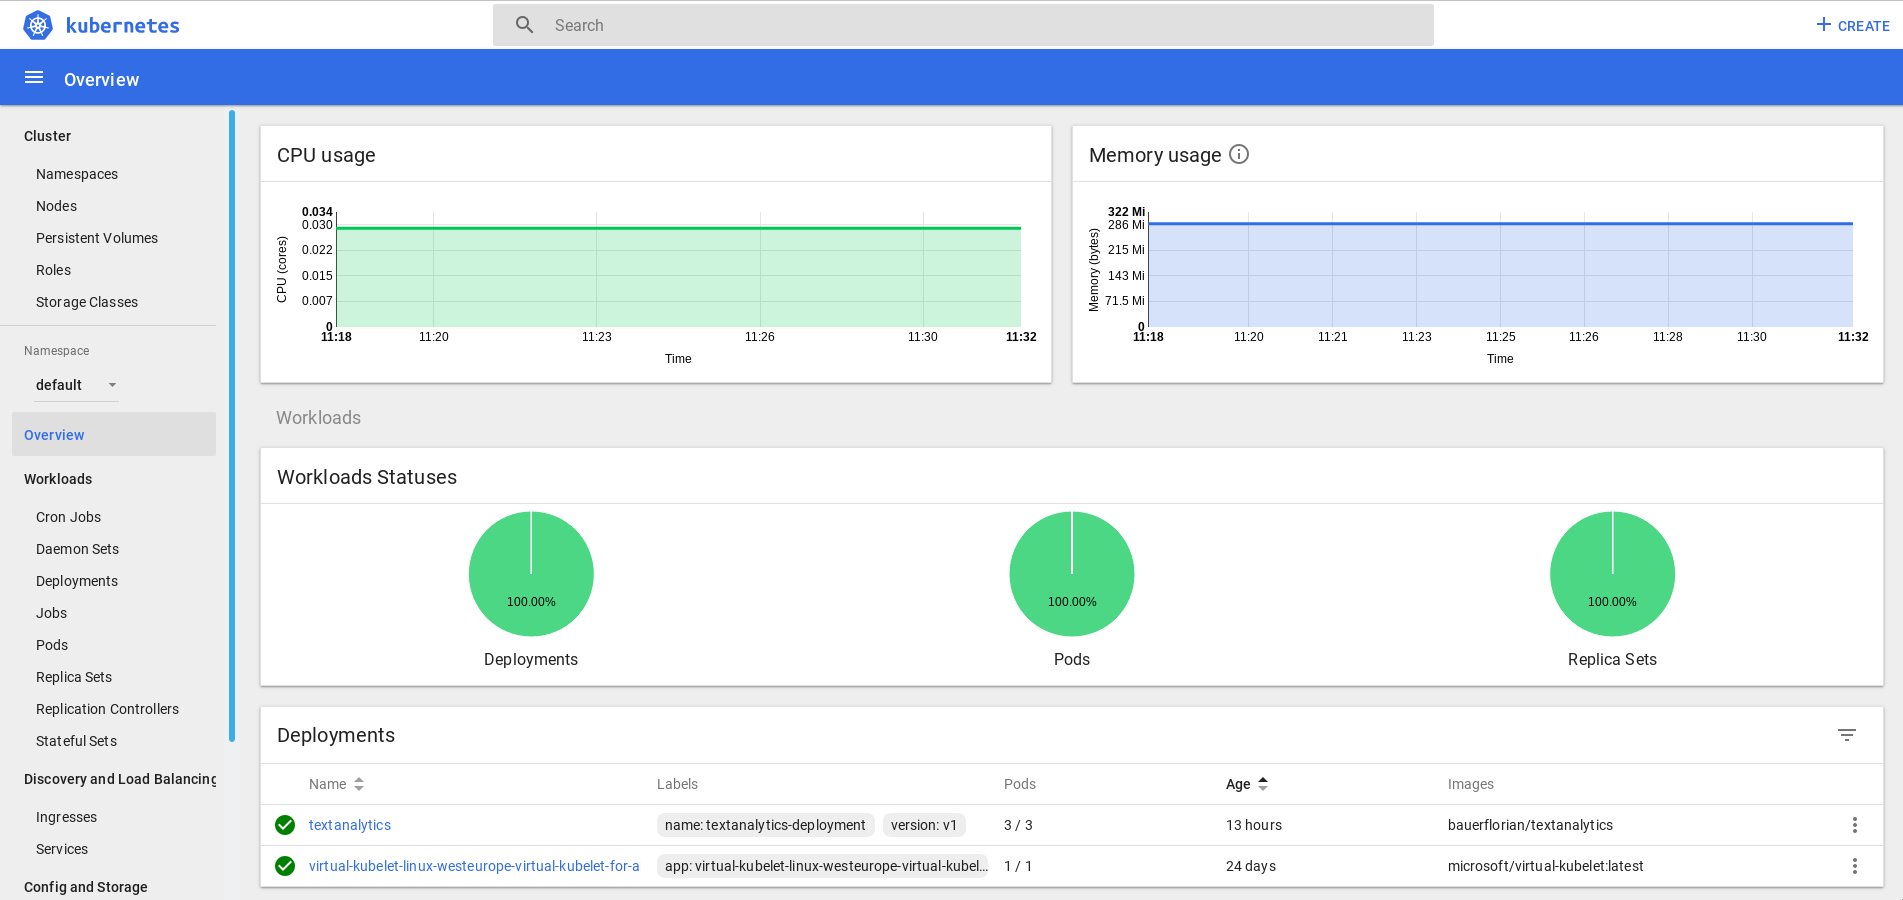
\includegraphics[width=170mm]{img/Kubernetes_Dashboard.png}
\caption{Kubernetes Dashboard}
\label{img:kubernetes-dashboard}
\end{figure*}

\section{Scalability}
\label{sec:scalability}
In case we will reach the point the web application gets more and more famous, and will be used more often the scalability of the application has a huge impact on the software experience and loading times. To build a good cloud application it should handle an unknown number of users parallel uploading and analyzing files without running into errors or bigger performance bottlenecks. In the rest of this section we discuss the creation of a scalable cloud application and show results of some load tests.

\subsection{Infrastructure}
As mentioned in \Cref{sec:system-architecture} all services are managed by the Kubernetes cluster.
The main advantage of using a Kubernetes cluster is scalability and loadbalancing. So if there is a high usage of the
existing resources the cluster can scale up by itself. In our case this might happen at peak times when a lot of people
are using the Text Analytica web service. Than the cluster creates more \textit{Pods} or \textit{Azure VM Nodes}, to handle the additional work without losing performance \cite{MicrosoftAzureKubernetesService}.

As we are using \textit{Virtual Kubelets}, we can achieve even faster up- and downscaling times
than with the pure Kubernetes cluster itself. This is due to the fact we do not need to wait on new VMs as already explained in \Cref{subsec:infra}.
\cite{MicrosoftVirtualNode}.

\subsection{Data storage}
The cloud application Text Analytica uses as storage an instance of Azure's \textit{Cosmos DB}. In the following part of this section we are discussing the scalability and consequently the regions and kinds of partitions of this database and what this means for our application.

There are two kinds of partitioning in \textit{Cosmos DB}: The logical partition, where all datasets or elements in a container have a similar property. Here the data itself and the data throughput is automatically, horizontally partitioned and scaled by Cosmos DB. Then there are the physical partitions. A number of logical partitions are assigned to one physical partition, which guarantees persistence and consistency of the data \cite{CosmosDBHorScal}.

It is possible to configure \textit{Cosmos DB} with multiple regions, which leads to a high availability as well (up to $99,999\%$)\cite{CosmosDBHA}.

\subsection{Service}
One of the main advantages using microservices is the opportunity of containerizing them. So you create and build for each microservices its own container. These containers you can create and also delete very fast and as you need them.
In terms of scalability this is a nice way adjusting the number of containers/services on demand.
This workflow of creating more containers if there are more needed is called \textit{horizontal scaling}. To manage this autoscaling for microservices container orchestration tools are used; in our case this is \textit{Kubernetes}.
\cite{GuideContainerClusters}
\cite{KubernetesScaling}
\cite{KubernetesAutoscaler}

\subsection{Monitoring and Load Testing}
To know how good a cloud application scales with an increasing amount of work respectively more users a load test is perfect for. We used the \textit{Azure Loadtest}, as this is an inbuild tool of the Azure Cloud Services and works efficiently for our use case.

In \Cref{img:loadtesting} there are the results of one of our load tests. In the figure there are four diagrams, for \textit{Performance}, \textit{Throughput}, \textit{Errors} and \textit{Tests}. This test lasted ten minutes and involved 700 virtual users. In the \textit{Errors} diagram can be seen there is no error, which means our application still works even under high usage. In the \textit{Performance} part there is the increasing user load and the increasing average response time as well as average page time. It follows our application has a good scaling rate, as the response time scales nearly linear with a fast performance. The \textit{Throughput} figure shows the pages/sec and requests/sec with increasing user load, and \textit{Tests} simply shows the tests/sec and average test time.

A useful tool for monitoring the Kubernetes cluster is the \textit{Kubernetes Dashboard}, which can be seen in \Cref{img:kubernetes-dashboard}. Here all important resources can be watched , e.g. number of working pods, CPU usage and memory usage. For debugging and in case of errors this tool was really helpful.

\section{Future improvements}
\label{sec:future-improvements}
\subsection{Infrastructure}
•	Split up microservices, front-end, back-end and analysis into separate containers, this would also allow for ingress to act as an application layer load balancer directing incoming traffic to the right service

•	Another possibility would be to go serverless, that is using PaaS and tools like Azure functions

•	Improve management of the kubernetes cluster by using popular open source projects like Istio.

\subsection{Service implementation}
•	Solve small bugs like missing ID in display

•	Add functionality like login, pdf, text recognition, more advanced analysis, save files and retrieve them, ...

•	Add / consider security measures, as of now there has been no focus on this

•	Extend the existing Continuous Delivery Pipeline and add test and dev stages to it.

\section{Conclusion}
\label{sec:conclusion}
conclusion...

\bibliographystyle{acm}
\bibliography{cw1-97059-97133}


\end{document}
